\documentclass[twoside]{book}

% Packages required by doxygen
\usepackage{fixltx2e}
\usepackage{calc}
\usepackage{doxygen}
\usepackage[export]{adjustbox} % also loads graphicx
\usepackage{graphicx}
\usepackage[utf8]{inputenc}
\usepackage{makeidx}
\usepackage{multicol}
\usepackage{multirow}
\PassOptionsToPackage{warn}{textcomp}
\usepackage{textcomp}
\usepackage[nointegrals]{wasysym}
\usepackage[table]{xcolor}

% Font selection
\usepackage[T1]{fontenc}
\usepackage[scaled=.90]{helvet}
\usepackage{courier}
\usepackage{amssymb}
\usepackage{sectsty}
\renewcommand{\familydefault}{\sfdefault}
\allsectionsfont{%
  \fontseries{bc}\selectfont%
  \color{darkgray}%
}
\renewcommand{\DoxyLabelFont}{%
  \fontseries{bc}\selectfont%
  \color{darkgray}%
}
\newcommand{\+}{\discretionary{\mbox{\scriptsize$\hookleftarrow$}}{}{}}

% Page & text layout
\usepackage{geometry}
\geometry{%
  a4paper,%
  top=2.5cm,%
  bottom=2.5cm,%
  left=2.5cm,%
  right=2.5cm%
}
\tolerance=750
\hfuzz=15pt
\hbadness=750
\setlength{\emergencystretch}{15pt}
\setlength{\parindent}{0cm}
\setlength{\parskip}{3ex plus 2ex minus 2ex}
\makeatletter
\renewcommand{\paragraph}{%
  \@startsection{paragraph}{4}{0ex}{-1.0ex}{1.0ex}{%
    \normalfont\normalsize\bfseries\SS@parafont%
  }%
}
\renewcommand{\subparagraph}{%
  \@startsection{subparagraph}{5}{0ex}{-1.0ex}{1.0ex}{%
    \normalfont\normalsize\bfseries\SS@subparafont%
  }%
}
\makeatother

% Headers & footers
\usepackage{fancyhdr}
\pagestyle{fancyplain}
\fancyhead[LE]{\fancyplain{}{\bfseries\thepage}}
\fancyhead[CE]{\fancyplain{}{}}
\fancyhead[RE]{\fancyplain{}{\bfseries\leftmark}}
\fancyhead[LO]{\fancyplain{}{\bfseries\rightmark}}
\fancyhead[CO]{\fancyplain{}{}}
\fancyhead[RO]{\fancyplain{}{\bfseries\thepage}}
\fancyfoot[LE]{\fancyplain{}{}}
\fancyfoot[CE]{\fancyplain{}{}}
\fancyfoot[RE]{\fancyplain{}{\bfseries\scriptsize Generated by Doxygen }}
\fancyfoot[LO]{\fancyplain{}{\bfseries\scriptsize Generated by Doxygen }}
\fancyfoot[CO]{\fancyplain{}{}}
\fancyfoot[RO]{\fancyplain{}{}}
\renewcommand{\footrulewidth}{0.4pt}
\renewcommand{\chaptermark}[1]{%
  \markboth{#1}{}%
}
\renewcommand{\sectionmark}[1]{%
  \markright{\thesection\ #1}%
}

% Indices & bibliography
\usepackage{natbib}
\usepackage[titles]{tocloft}
\setcounter{tocdepth}{3}
\setcounter{secnumdepth}{5}
\makeindex

% Hyperlinks (required, but should be loaded last)
\usepackage{ifpdf}
\ifpdf
  \usepackage[pdftex,pagebackref=true]{hyperref}
\else
  \usepackage[ps2pdf,pagebackref=true]{hyperref}
\fi
\hypersetup{%
  colorlinks=true,%
  linkcolor=blue,%
  citecolor=blue,%
  unicode%
}

% Custom commands
\newcommand{\clearemptydoublepage}{%
  \newpage{\pagestyle{empty}\cleardoublepage}%
}

\usepackage{caption}
\captionsetup{labelsep=space,justification=centering,font={bf},singlelinecheck=off,skip=4pt,position=top}

%===== C O N T E N T S =====

\begin{document}

% Titlepage & ToC
\hypersetup{pageanchor=false,
             bookmarksnumbered=true,
             pdfencoding=unicode
            }
\pagenumbering{alph}
\begin{titlepage}
\vspace*{7cm}
\begin{center}%
{\Large Reference Manual}\\
\vspace*{1cm}
{\large Generated by Doxygen 1.8.14}\\
\end{center}
\end{titlepage}
\clearemptydoublepage
\pagenumbering{roman}
\tableofcontents
\clearemptydoublepage
\pagenumbering{arabic}
\hypersetup{pageanchor=true}

%--- Begin generated contents ---
\chapter{Description}
\label{index}\hypertarget{index}{}S\+EP Projekt zu Flashkaskaden 
\chapter{Namespace Index}
\section{Namespace List}
Here is a list of all namespaces with brief descriptions\+:\begin{DoxyCompactList}
\item\contentsline{section}{\mbox{\hyperlink{namespace_ui}{Ui}} }{\pageref{namespace_ui}}{}
\end{DoxyCompactList}

\chapter{Hierarchical Index}
\section{Class Hierarchy}
This inheritance list is sorted roughly, but not completely, alphabetically\+:\begin{DoxyCompactList}
\item \contentsline{section}{cascade$<$ TS, NP, NS, TP $>$}{\pageref{classcascade}}{}
\item \contentsline{section}{L\+I\+N\+E\+A\+R\+\_\+\+S\+O\+L\+V\+ER$<$ TA, N, Tb, Tx $>$}{\pageref{class_l_i_n_e_a_r___s_o_l_v_e_r}}{}
\begin{DoxyCompactList}
\item \contentsline{section}{LU$<$ TA, N, Tb, Tx $>$}{\pageref{class_l_u}}{}
\item \contentsline{section}{QR$<$ TA, N, Tb, Tx $>$}{\pageref{class_q_r}}{}
\end{DoxyCompactList}
\item \contentsline{section}{L\+I\+N\+E\+A\+R\+\_\+\+S\+O\+L\+V\+ER$<$ TS, NS $>$}{\pageref{class_l_i_n_e_a_r___s_o_l_v_e_r}}{}
\item \contentsline{section}{L\+I\+N\+E\+A\+R\+\_\+\+S\+Y\+S\+T\+EM$<$ TA, N, Tb, Tx $>$}{\pageref{class_l_i_n_e_a_r___s_y_s_t_e_m}}{}
\item \contentsline{section}{Module$<$ TS, NP, NS, TP $>$}{\pageref{class_module}}{}
\item \contentsline{section}{Module$<$$>$}{\pageref{class_module}}{}
\begin{DoxyCompactList}
\item \contentsline{section}{Flash$<$ TS, NP, NS, TP $>$}{\pageref{class_flash}}{}
\end{DoxyCompactList}
\item \contentsline{section}{M\+O\+D\+U\+L\+E\+N\+E\+W\+T\+ON$<$ TS, NP, NS, TP $>$}{\pageref{class_m_o_d_u_l_e_n_e_w_t_o_n}}{}
\item \contentsline{section}{N\+O\+N\+L\+I\+N\+E\+A\+R\+\_\+\+S\+O\+L\+V\+ER$<$ TS, NP, NS, TP $>$}{\pageref{class_n_o_n_l_i_n_e_a_r___s_o_l_v_e_r}}{}
\begin{DoxyCompactList}
\item \contentsline{section}{N\+E\+W\+T\+ON$<$ TS, NP, NS, TP $>$}{\pageref{class_n_e_w_t_o_n}}{}
\end{DoxyCompactList}
\item \contentsline{section}{N\+O\+N\+L\+I\+N\+E\+A\+R\+\_\+\+S\+Y\+S\+T\+EM$<$ TS, NP, NS, TP $>$}{\pageref{class_n_o_n_l_i_n_e_a_r___s_y_s_t_e_m}}{}
\item Q\+Main\+Window\begin{DoxyCompactList}
\item \contentsline{section}{Main\+Window}{\pageref{class_main_window}}{}
\end{DoxyCompactList}
\item \contentsline{section}{Test\+Class}{\pageref{class_test_class}}{}
\end{DoxyCompactList}

\chapter{Class Index}
\section{Class List}
Here are the classes, structs, unions and interfaces with brief descriptions\+:\begin{DoxyCompactList}
\item\contentsline{section}{\mbox{\hyperlink{classcascade}{cascade$<$ Real\+Type $>$}} \\*Enthält alle Flashes }{\pageref{classcascade}}{}
\item\contentsline{section}{\mbox{\hyperlink{class_c_a_s_c_a_d_e_e_s_o}{C\+A\+S\+C\+A\+D\+E\+E\+SO}} }{\pageref{class_c_a_s_c_a_d_e_e_s_o}}{}
\item\contentsline{section}{\mbox{\hyperlink{class_flash}{Flash$<$ Real\+Type $>$}} \\*Flashmodul }{\pageref{class_flash}}{}
\item\contentsline{section}{\mbox{\hyperlink{class_l_i_n_e_a_r___s_o_l_v_e_r}{L\+I\+N\+E\+A\+R\+\_\+\+S\+O\+L\+V\+E\+R$<$ T\+A, N, Tb, Tx $>$}} }{\pageref{class_l_i_n_e_a_r___s_o_l_v_e_r}}{}
\item\contentsline{section}{\mbox{\hyperlink{class_l_i_n_e_a_r___s_y_s_t_e_m}{L\+I\+N\+E\+A\+R\+\_\+\+S\+Y\+S\+T\+E\+M$<$ T\+A, N, Tb, Tx $>$}} \\*Lineare Systeme Basierend auf \mbox{\hyperlink{lin__sys_8h}{lin\+\_\+sys.\+h}} von Uwe Naumann }{\pageref{class_l_i_n_e_a_r___s_y_s_t_e_m}}{}
\item\contentsline{section}{\mbox{\hyperlink{class_l_u}{L\+U$<$ T\+A, N, Tb, Tx $>$}} }{\pageref{class_l_u}}{}
\item\contentsline{section}{\mbox{\hyperlink{class_module}{Module$<$ Real\+Type $>$}} \\*Akstrakte Klasse für allgemeine Bauteile }{\pageref{class_module}}{}
\item\contentsline{section}{\mbox{\hyperlink{class_n_e_w_t_o_n}{N\+E\+W\+T\+O\+N$<$ T\+S, N\+P, N\+S, T\+P $>$}} }{\pageref{class_n_e_w_t_o_n}}{}
\item\contentsline{section}{\mbox{\hyperlink{class_n_o_n_l_i_n_e_a_r___s_o_l_v_e_r}{N\+O\+N\+L\+I\+N\+E\+A\+R\+\_\+\+S\+O\+L\+V\+E\+R$<$ T\+S, N\+P, N\+S, T\+P $>$}} }{\pageref{class_n_o_n_l_i_n_e_a_r___s_o_l_v_e_r}}{}
\item\contentsline{section}{\mbox{\hyperlink{class_n_o_n_l_i_n_e_a_r___s_y_s_t_e_m}{N\+O\+N\+L\+I\+N\+E\+A\+R\+\_\+\+S\+Y\+S\+T\+E\+M$<$ T\+S, N\+P, N\+S, T\+P $>$}} \\*Nichtlineare Systeme Basierend auf \mbox{\hyperlink{nonlin__sys_8h}{nonlin\+\_\+sys.\+h}} von Uwe Naumann }{\pageref{class_n_o_n_l_i_n_e_a_r___s_y_s_t_e_m}}{}
\item\contentsline{section}{\mbox{\hyperlink{class_q_r}{Q\+R$<$ T\+A, N, Tb, Tx $>$}} }{\pageref{class_q_r}}{}
\item\contentsline{section}{\mbox{\hyperlink{class_world_machine}{World\+Machine}} \\*C++ -\/ Q\+ML Schnittstelle Organisiert die Kaskade und das G\+UI }{\pageref{class_world_machine}}{}
\end{DoxyCompactList}

\chapter{File Index}
\section{File List}
Here is a list of all files with brief descriptions\+:\begin{DoxyCompactList}
\item\contentsline{section}{\mbox{\hyperlink{cascade_8h}{cascade.\+h}} \\*Enthält alle \mbox{\hyperlink{class_module}{Module}} }{\pageref{cascade_8h}}{}
\item\contentsline{section}{\mbox{\hyperlink{flash_8h}{flash.\+h}} \\*\mbox{\hyperlink{class_flash}{Flash}} als Erweiterung des Moduls }{\pageref{flash_8h}}{}
\item\contentsline{section}{\mbox{\hyperlink{lin__sys_8h}{lin\+\_\+sys.\+h}} \\*Lineare Systeme }{\pageref{lin__sys_8h}}{}
\item\contentsline{section}{\mbox{\hyperlink{main_8cpp}{main.\+cpp}} \\*Main funcion }{\pageref{main_8cpp}}{}
\item\contentsline{section}{\mbox{\hyperlink{mainwindow_8cpp}{mainwindow.\+cpp}} \\*Hauptfenster }{\pageref{mainwindow_8cpp}}{}
\item\contentsline{section}{\mbox{\hyperlink{mainwindow_8h}{mainwindow.\+h}} \\*Hauptfenster }{\pageref{mainwindow_8h}}{}
\item\contentsline{section}{\mbox{\hyperlink{module_8h}{module.\+h}} \\*Basismodul }{\pageref{module_8h}}{}
\item\contentsline{section}{\mbox{\hyperlink{nonlin__sys_8h}{nonlin\+\_\+sys.\+h}} \\*Nichtlineare Systeme }{\pageref{nonlin__sys_8h}}{}
\item\contentsline{section}{\mbox{\hyperlink{testclass_8h}{testclass.\+h}} }{\pageref{testclass_8h}}{}
\end{DoxyCompactList}

\chapter{Namespace Documentation}
\hypertarget{namespace_ui}{}\section{Ui Namespace Reference}
\label{namespace_ui}\index{Ui@{Ui}}

\chapter{Class Documentation}
\hypertarget{class_main_window}{}\section{Main\+Window Class Reference}
\label{class_main_window}\index{Main\+Window@{Main\+Window}}


Hauptfenster.  




{\ttfamily \#include $<$mainwindow.\+h$>$}



Inheritance diagram for Main\+Window\+:\nopagebreak
\begin{figure}[H]
\begin{center}
\leavevmode
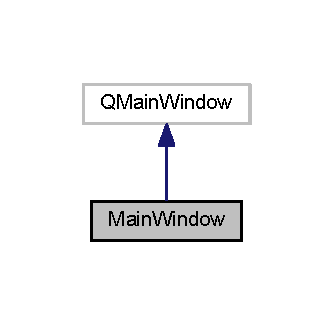
\includegraphics[width=160pt]{class_main_window__inherit__graph}
\end{center}
\end{figure}


Collaboration diagram for Main\+Window\+:\nopagebreak
\begin{figure}[H]
\begin{center}
\leavevmode
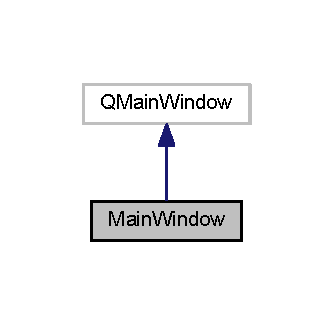
\includegraphics[width=160pt]{class_main_window__coll__graph}
\end{center}
\end{figure}
\subsection*{Public Member Functions}
\begin{DoxyCompactItemize}
\item 
\mbox{\hyperlink{class_main_window_a8b244be8b7b7db1b08de2a2acb9409db}{Main\+Window}} (Q\+Widget $\ast$parent=0)
\item 
\mbox{\hyperlink{class_main_window_ae98d00a93bc118200eeef9f9bba1dba7}{$\sim$\+Main\+Window}} ()
\item 
void \mbox{\hyperlink{class_main_window_a962b966d1e81982b7b9da86f0df0bbc1}{add\+Button}} ()
\end{DoxyCompactItemize}


\subsection{Detailed Description}
Hauptfenster. 

\subsection{Constructor \& Destructor Documentation}
\mbox{\Hypertarget{class_main_window_a8b244be8b7b7db1b08de2a2acb9409db}\label{class_main_window_a8b244be8b7b7db1b08de2a2acb9409db}} 
\index{Main\+Window@{Main\+Window}!Main\+Window@{Main\+Window}}
\index{Main\+Window@{Main\+Window}!Main\+Window@{Main\+Window}}
\subsubsection{\texorpdfstring{Main\+Window()}{MainWindow()}}
{\footnotesize\ttfamily Main\+Window\+::\+Main\+Window (\begin{DoxyParamCaption}\item[{Q\+Widget $\ast$}]{parent = {\ttfamily 0} }\end{DoxyParamCaption})\hspace{0.3cm}{\ttfamily [explicit]}}

\mbox{\Hypertarget{class_main_window_ae98d00a93bc118200eeef9f9bba1dba7}\label{class_main_window_ae98d00a93bc118200eeef9f9bba1dba7}} 
\index{Main\+Window@{Main\+Window}!````~Main\+Window@{$\sim$\+Main\+Window}}
\index{````~Main\+Window@{$\sim$\+Main\+Window}!Main\+Window@{Main\+Window}}
\subsubsection{\texorpdfstring{$\sim$\+Main\+Window()}{~MainWindow()}}
{\footnotesize\ttfamily Main\+Window\+::$\sim$\+Main\+Window (\begin{DoxyParamCaption}{ }\end{DoxyParamCaption})}



\subsection{Member Function Documentation}
\mbox{\Hypertarget{class_main_window_a962b966d1e81982b7b9da86f0df0bbc1}\label{class_main_window_a962b966d1e81982b7b9da86f0df0bbc1}} 
\index{Main\+Window@{Main\+Window}!add\+Button@{add\+Button}}
\index{add\+Button@{add\+Button}!Main\+Window@{Main\+Window}}
\subsubsection{\texorpdfstring{add\+Button()}{addButton()}}
{\footnotesize\ttfamily void Main\+Window\+::add\+Button (\begin{DoxyParamCaption}{ }\end{DoxyParamCaption})}

Here is the caller graph for this function\+:\nopagebreak
\begin{figure}[H]
\begin{center}
\leavevmode
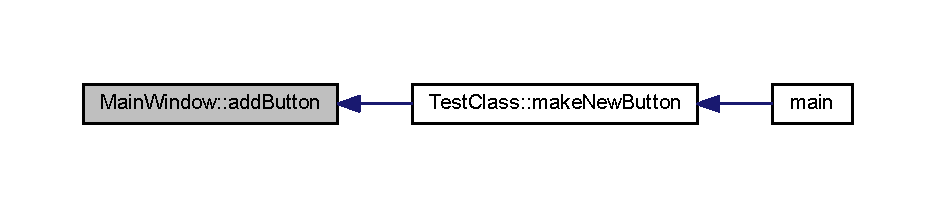
\includegraphics[width=350pt]{class_main_window_a962b966d1e81982b7b9da86f0df0bbc1_icgraph}
\end{center}
\end{figure}


The documentation for this class was generated from the following files\+:\begin{DoxyCompactItemize}
\item 
\mbox{\hyperlink{mainwindow_8h}{mainwindow.\+h}}\item 
\mbox{\hyperlink{mainwindow_8cpp}{mainwindow.\+cpp}}\end{DoxyCompactItemize}

\chapter{File Documentation}
\hypertarget{main_8cpp}{}\section{main.\+cpp File Reference}
\label{main_8cpp}\index{main.\+cpp@{main.\+cpp}}


Programminitiation.  


{\ttfamily \#include \char`\"{}World\+Machine.\+h\char`\"{}}\newline
{\ttfamily \#include $<$Q\+Gui\+Application$>$}\newline
{\ttfamily \#include $<$Qt\+Qml/\+Q\+Qml\+Application\+Engine$>$}\newline
{\ttfamily \#include $<$Qt\+Qml/\+Q\+Qml\+Engine$>$}\newline
Include dependency graph for main.\+cpp\+:\nopagebreak
\begin{figure}[H]
\begin{center}
\leavevmode
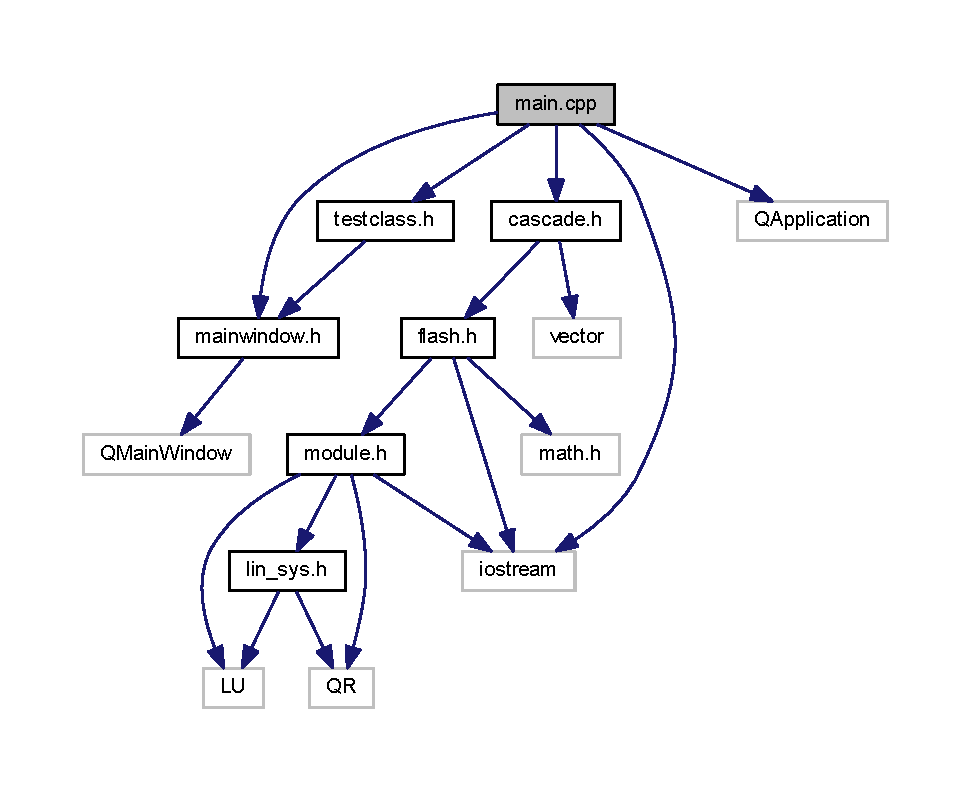
\includegraphics[width=350pt]{main_8cpp__incl}
\end{center}
\end{figure}
\subsection*{Functions}
\begin{DoxyCompactItemize}
\item 
int \mbox{\hyperlink{main_8cpp_a0ddf1224851353fc92bfbff6f499fa97}{main}} (int argc, char $\ast$argv\mbox{[}$\,$\mbox{]})
\end{DoxyCompactItemize}


\subsection{Detailed Description}
Programminitiation. 


\begin{DoxyParams}{Parameters}
{\em argc} & dummy \\
\hline
{\em argv} & dummy \\
\hline
\end{DoxyParams}


\subsection{Function Documentation}
\mbox{\Hypertarget{main_8cpp_a0ddf1224851353fc92bfbff6f499fa97}\label{main_8cpp_a0ddf1224851353fc92bfbff6f499fa97}} 
\index{main.\+cpp@{main.\+cpp}!main@{main}}
\index{main@{main}!main.\+cpp@{main.\+cpp}}
\subsubsection{\texorpdfstring{main()}{main()}}
{\footnotesize\ttfamily int main (\begin{DoxyParamCaption}\item[{int}]{argc,  }\item[{char $\ast$}]{argv\mbox{[}$\,$\mbox{]} }\end{DoxyParamCaption})}


\hypertarget{mainwindow_8cpp}{}\section{mainwindow.\+cpp File Reference}
\label{mainwindow_8cpp}\index{mainwindow.\+cpp@{mainwindow.\+cpp}}


Main Window.  


{\ttfamily \#include \char`\"{}mainwindow.\+h\char`\"{}}\newline
{\ttfamily \#include \char`\"{}ui\+\_\+mainwindow.\+h\char`\"{}}\newline
Include dependency graph for mainwindow.\+cpp\+:\nopagebreak
\begin{figure}[H]
\begin{center}
\leavevmode
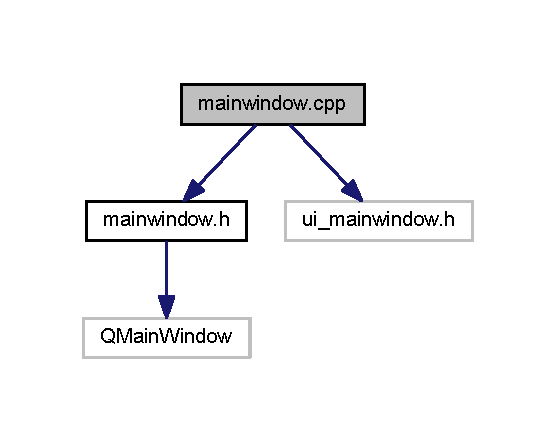
\includegraphics[width=267pt]{mainwindow_8cpp__incl}
\end{center}
\end{figure}


\subsection{Detailed Description}
Main Window. 


\begin{DoxyParams}{Parameters}
{\em parent} & \\
\hline
\end{DoxyParams}

\hypertarget{mainwindow_8h}{}\section{mainwindow.\+h File Reference}
\label{mainwindow_8h}\index{mainwindow.\+h@{mainwindow.\+h}}


Hauptfenster.  


{\ttfamily \#include $<$Q\+Main\+Window$>$}\newline
Include dependency graph for mainwindow.\+h\+:\nopagebreak
\begin{figure}[H]
\begin{center}
\leavevmode
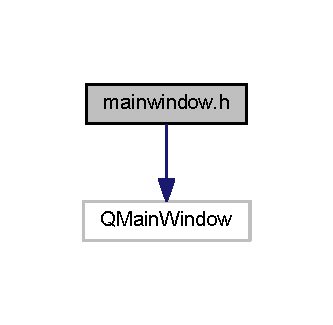
\includegraphics[width=160pt]{mainwindow_8h__incl}
\end{center}
\end{figure}
This graph shows which files directly or indirectly include this file\+:\nopagebreak
\begin{figure}[H]
\begin{center}
\leavevmode
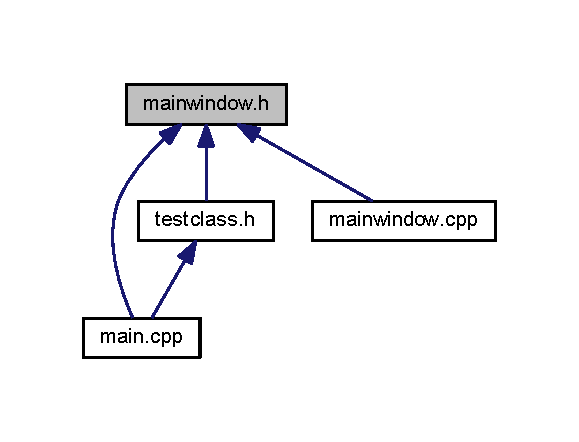
\includegraphics[width=278pt]{mainwindow_8h__dep__incl}
\end{center}
\end{figure}
\subsection*{Classes}
\begin{DoxyCompactItemize}
\item 
class \mbox{\hyperlink{class_main_window}{Main\+Window}}
\begin{DoxyCompactList}\small\item\em Hauptfenster. \end{DoxyCompactList}\end{DoxyCompactItemize}
\subsection*{Namespaces}
\begin{DoxyCompactItemize}
\item 
 \mbox{\hyperlink{namespace_ui}{Ui}}
\end{DoxyCompactItemize}


\subsection{Detailed Description}
Hauptfenster. 


%--- End generated contents ---

% Index
\backmatter
\newpage
\phantomsection
\clearemptydoublepage
\addcontentsline{toc}{chapter}{Index}
\printindex

\end{document}
